\section{Results}
\label{sec:results}

We start by describing the results for each study in detail, before proceeding to summarise and discuss the observed effects. All the studies results are available online for replication purposes~\cite{Data-Results}.

\subsection{Experimental Simulation}
\label{sec:expResults}

%demographics
The participant set encompasses graduates in Computer Science or Software Engineering -- either working in industry (41.6\%) or M.Sc. and Ph.D. candidates (58.4\%).
%table
In Table~\ref{tab:results} we summarise the results from the 24 trials, from which five -- 21\% -- were delivered with at least one fault detected by our test cases.
%individual results
All participants assigned to textual specifications in Javadoc delivered correct programs.
By contrast, half of the programs delivered by participants using APIs with formal contracts were faulty (four out of eight).
One faulty program was delivered by a participant assigned to \contractjdoc{}.
%task
Regarding task, faults were mostly in API implementations -- four of them, if compared with only one in API clients.
% source code correct
%Javadoc and \contractjdoc{} were the only documenting approaches in which all participants were able to produce a code satisfying the oracle (respecting the restrictions available in the comments). On the other hand, there was one case developed by following the JML documenting approach in which the contract is not satisfied by the implementation.



\begin{table}
\centering
\caption{Experimental results, for each treatment (textual Javadoc \emph{JavaDoc}, \contractjdoc{} \emph{ContJDoc} and formal contracts \emph{Formal}. For each API (Queue or Stack) and Task (\emph{Cli} if a client for the API was implemented, \emph{Sup} if an implementation for the API was provided), participants are listed (\emph{Part}) along with the result (\emph{Res}) from our test cases.}
\label{tab:results}
\begin{tabular}{|l|l||l|l||l|l||l|l|} 
\cline{3-8}
\multicolumn{1}{l}{} &              & \multicolumn{2}{l||}{\textbf{JavaDoc }} & \multicolumn{2}{l||}{\textbf{ContJDoc }} & \multicolumn{2}{l|}{\textbf{Formal}}  \\ 
\hline
\uline{DataStr}      & \uline{Task} & Part & Res                              & Part & Res                                & Part & Res                             \\ 
\hline\hline
\uline{Queue}        & \uline{Cli}  & p9   & \greencheck       & p11  & \greencheck                                    & p7   & \greencheck                                 \\
                     & \uline{Cli}  & p10  & \greencheck                                 & p12  & \greencheck                                    & p8   & \greencheck                                \\
                     & \uline{Sup}  & p21  & \greencheck                                 & p23  & \greencheck                                    & p19  &  \greencheck                               \\
                     & \uline{Sup}  & p22  & \greencheck                                 & p24  & \greencheck                                    & p20  &  \redcross                               \\ 
\hline\hline
\uline{Stack}        & \uline{Cli}  & p3   & \greencheck                                 & p5   & \greencheck                                    & p1   & \redcross                                 \\
                     & \uline{Cli}  & p4   & \greencheck                                 & p6   & \greencheck                                    & p2   & \greencheck                                 \\
                     & \uline{Sup}  & p15  & \greencheck                                 & p17  & \redcross                                    & p13  & \redcross                                \\
                     & \uline{Sup}  & p16  & \greencheck                                 & p18  & \greencheck                                    & p14  & \redcross                                \\
\hline
\end{tabular}
\end{table}

%faults
Table~\ref{tab:faults} details some of the results from participants' submissions, including the faults detected by the test cases. After a detailed analysis of the programs, we classified each fault regarding the violated contract. 
%clients
\emph{All clients fulfilled the specified pre-conditions for calling API methods} -- p1's client raises an exception which was incompatible with the method's post-condition.
%suppliers
\emph{All four faults unveiled in API implementations resulted from failing to satisfy the specified post-condition} in methods removing data from the given structure (two on \texttt{Stack.pop} and two on \texttt{Queue.remove}).

\begin{table}
\centering
\caption{Reason (fault) for failures in participants' results}
\label{tab:faults}
\begin{adjustbox}{width=\textwidth}
\begin{tabular}{|l|l|l|l|} 
\hline
\multicolumn{4}{|l|}{\textbf{ContractJDoc }}                                                                                                                                                                    \\ 
\hline
p17                                        & Stack                             & Sup                                & Post-condition violation on method \texttt{remove}                                    \\ 
\hline
\multicolumn{4}{|l|}{\textbf{Formal contracts} }                                                                                                                                                                \\ 
\hline
p1                                         & Stack                             & Cli                                & Failure to expect correct exceptions from Post-condition on method \texttt{removeAccountTop}    \\ 
\hline
p13                                        & Stack                             & Sup                                & Post-condition violation on method \texttt{pop}     \\ 
\hline
p14                                        & Stack                             & Sup                                & Post-condition violation on method \texttt{pop}     \\ 
\hline
p20                                        & Queue                             & Sup                                & Post-condition violation on method \texttt{remove}  \\ 
\hline\hline
\multicolumn{1}{|c|}{\textbf{Part}} & \multicolumn{1}{c|}{\textbf{API}} & \multicolumn{1}{c|}{\textbf{Task}} & \multicolumn{1}{c|}{\textbf{Type of~Fault}}                                               \\
\hline
\end{tabular}
\end{adjustbox}
\end{table}

After they submitted the programs, we asked participants about understandability of the API specifications, using a Likert-like scale which ranges from 1 (less understandable) to 5 (very understandable). The results for 24 answers are summarised in Figure~\ref{fig:ExpAnswersTotal}, in which assessments are spread between 3 and 5. Most participants evaluated understandability as 4 (58\%).

\begin{figure*}
\centering
\begin{subfigure}{.32\textwidth}
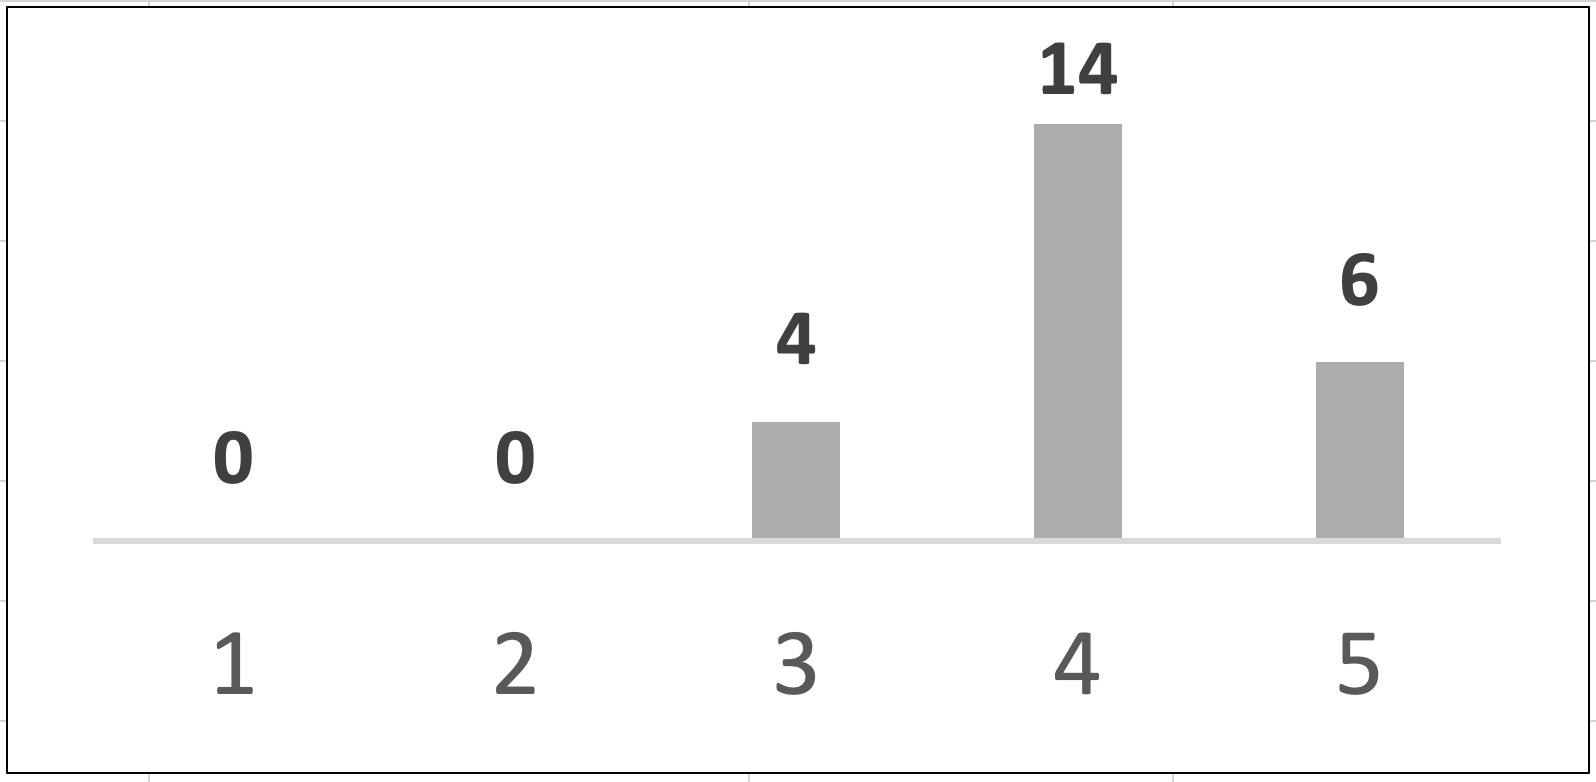
\includegraphics[width=1\textwidth]{figs/ExpAnswersTotal.png}
\caption{Total Results.}
\label{fig:ExpAnswersTotal}
\end{subfigure}
\begin{subfigure}{.33\textwidth}
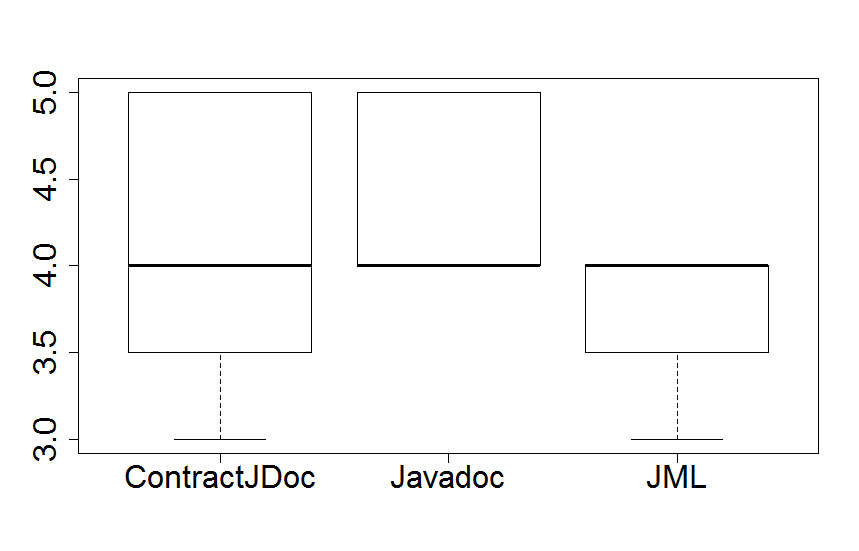
\includegraphics[width=1\linewidth]{figs/boxplotApproachesEmpiricalStudy}
\caption{Results by approach.}
\label{fig:approachesEmpirical}
\end{subfigure}
\begin{subfigure}{.33\textwidth}
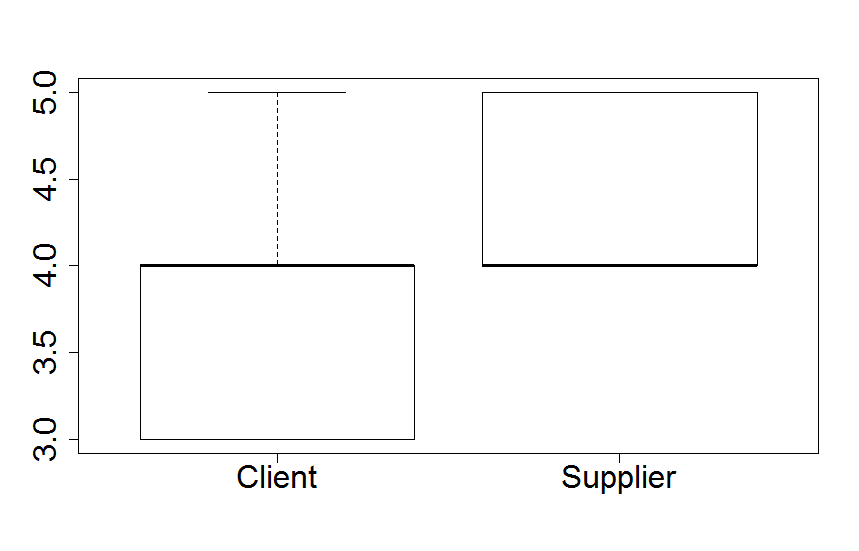
\includegraphics[width=1\linewidth]{figs/boxplotTasksEmpiricalStudy}
\caption{Results by task.}
\label{fig:tasksEmpirical}
\end{subfigure}
\caption{Results from Understandability Assessment of API specifications, as Perceived from Participants.}
\label{fig:empiricalResults}
\end{figure*}

%perspectives
Assuming a distinct perspective, we grouped understandability assessments by the assigned documentation approach and task -- Figures~\ref{fig:approachesEmpirical} and~\ref{fig:tasksEmpirical}, respectively, depict their distribution using boxplots.
%doc approach
The assessments for Javadoc APIs are all above the median ($4$), while \contractjdoc{} assessments fluctuate around that median value. Formal contracts, in turn, were all assessed as $3$ or $4$.  
% stats
Nevertheless, statistical tests (in this case, the Kruskal-Wallis non-parametric test) showed no difference between the groups (p-value = $0.15$, 95\% confidence level).
%task
Concerning the task performed by the developers, raw data shows a slightly higher understandability by participants assigned to supplier tasks. Still, the Wilcoxon rank sum test~\cite{statistical} reported no significant difference (p-value = 0.07, for confidence level of 95\%).

%qualitative results
Furthermore, we asked the participants, with an open-ended question, to provide comments on their tasks.
The quotes were organised in 11 categories, which are presented in Table~\ref{tab:categories}, in conjunction with the number of quotes; one quote may be classified in more than one category. Three participants did not provide an answer.

%on the results
%seven
We found that most quotes either value the specifications or suggest the contracts should have been stronger (seven each). As an example of the latter, p6, which was assigned a \contractjdoc{} API, wrote: \emph{"I hesitated over the \texttt{pop} method, due to its exception; there should be more information about the exception to be thrown in each case"}. 
%four
Others made explicit suggestions on how the specification should be, from their previous understanding of Queue and Stack APIs.
%other
Interestingly, we found a few quotes that expressed total trust in the contracts, dismissing defensive programming as advocated by the Design by Contract methodology ~\cite{dbc}.
Another category encompasses quotes that remark how the Javadoc text around the contract expressions helped them to understand the API specification. 

\begin{table}
\centering
\caption{Categories in Participants' quotes}
\label{tab:categories}
\begin{tabular}{|l|r|} 
\hline
\textbf{Category description}                & \multicolumn{1}{l|}{\textbf{\#quotes}}  \\ 
\hline\hline
Specifications were clear and understandable & 7                                       \\ 
\hline
Specifications were vague                    & 7                                       \\ 
\hline
Suggestions to change the specification      & 4                                       \\ 
\hline
The surrounding text helped understanding    & 2                                       \\ 
\hline
Total trust in the contracts                 & 2                                       \\ 
\hline
Contracts were ignored                       & 1                                       \\ 
\hline
Hard to read the logic                       & 1                                       \\ 
\hline
Questions about the task                     & 1                                       \\ 
\hline
Text was confusing                           & 1                                       \\
\hline
\end{tabular}
\end{table}


\subsection{Judgment Survey}
\label{sec:surveyResults}

%survey description
As a follow-up, we showed three versions of the Stack API as a web survey, asking questions about those approaches to contract specifications; we suggested respondents play the client role of the API as if they were about to call its methods.
%questions
Respondents were asked to assess understandability of each approach (again, using a 1--5 Likert scale), in addition to providing a verdict asking which approach they think is the most understandable as an API specification. For this, they were given three options -- one for each contract style -- and a fourth, neutral option.

%general results
From the universe of developers who received the invitation, answers from 142 Java developers were considered valid.
%demographics
%students and professionals
From those, 51 are graduate professionals (36\%), and 91 are undergraduate and graduate students in computer-related degrees (64\%).
%experience
Having some experience with Java was a requirement for being a participant; more than 73\% (105) have experience with either open source or industrial projects. Likewise, 74\% (105) of the respondents declared to have more than one year of Java programming.
%contract experience.
Regarding formal contract languages for specifying APIs (Eiffel, JML or similar), most respondents -- 67\% -- had no previous experience. 


%results - Javadoc is the simplest
Concerning the survey answers, Figure \ref{fig:understand} shows 50.7\% (72) of the respondents chose Javadoc as the most straightforward approach to understanding the provided API specification. 
%contractjdoc em JML
While only 11 (7\%) chose formal contracts as the most understandable approach and 18 (12\%) were indifferent, an almost one-third of the respondents (41, almost 29\%) chose the mix of text and contract expressions -- \contractjdoc{}.


\begin{figure*}
\centering
\begin{subfigure}{.45\textwidth}
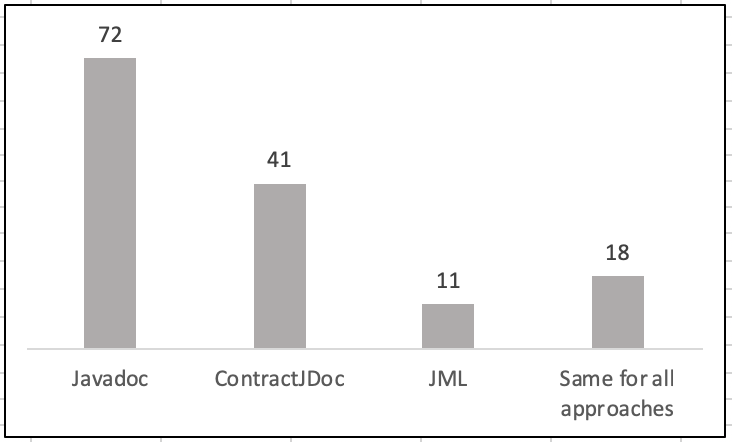
\includegraphics[width=0.8\linewidth]{figs/mostUnderstandable.png}
\caption{Surveyed Verdicts on Understandability.}
\label{fig:understand}
\end{subfigure}
\begin{subfigure}{.48\textwidth}
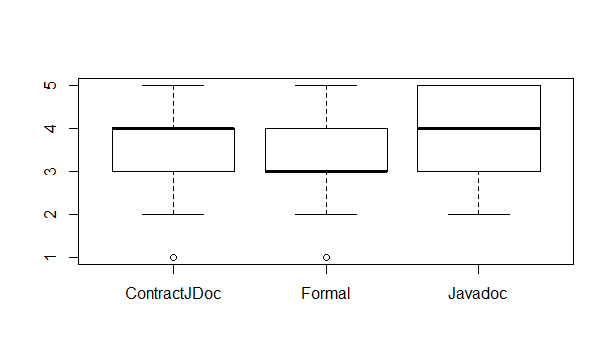
\includegraphics[width=1\linewidth]{figs/boxplotApproachesSurveyStudy}
\caption{Assessment for Each Contract Style.}
\label{fig:surveyResults}
\end{subfigure}
\caption{Results from the Judgement Survey.}
\label{fig:survey}
\end{figure*}


% individual answers to each approach
After being presented with three versions of the same API, the distribution of assessments for each contract style is showed in Figure~\ref{fig:surveyResults}.
%explain visual
Answers for Javadoc and \contractjdoc{} were distributed around a median of $4.0$; for the first, assessments range from $3$ to $5$, while assesments for the latter were no higher than $4$.
Likewise, formal contracts were evaluated with $4$ the highest, however with $3$ with centre value. 

\begin{figure}
\centering
\end{figure}


%statistical results
Differently from the experimental simulation from Section~\ref{sec:expResults}, statistical tests show a \emph{significant difference between the assessments}. The application of One-way Analysis of Variance (ANOVA), which is robust enough for non-normal distributions~\cite{statistical}, detected a distinction between the three groups of answers (p-value $<$ 0.05). 
To estimate the assessment differences between each pair of groups, we applied post hoc analysis -- Tukey HSD with Bonferroni correction~\cite{statistical}. Cohen's effect sizes are shown in Table~\ref{tab:effect}, expressing significant difference between all styles. Using formal contracts as baseline, \contractjdoc{} presented greater understandability grades by a medium effect size; the same with Javadoc, but with a large effect size. With \contractjdoc{} as baseline, the effect of Javadoc over \contractjdoc{} is smaller, but also medium (d=$0.343$).

\begin{table}
\centering
\caption{Effect sizes (Cohen) from Tukey HSD with Bonferroni correction}
\label{tab:effect}
\begin{tabular}{l|r} 
\toprule
\textbf{Group Pairs}                                                & \textbf{Effect size}  \\ 
\toprule
Javadoc $\rightarrow$ \contractjdoc{} & 0.343                 \\
\contractjdoc{} $\rightarrow$ formal  & 0.516                 \\
Javadoc $\rightarrow$ formal          & 0.902                \\
\hline
\end{tabular}
\end{table}



%effect sizes

% cohen.d(javadocSurvey$Difficulty, contractJDocSurvey$Difficulty)
% 
% Cohen's d
% 
% d estimate: 0.3429443 (small)
% 95 percent confidence interval:
%     lower     upper 
% 0.1076259 0.5782627 
% > cohen.d(contractJDocSurvey$Difficulty, jmlSurvey$Difficulty)
% 
% Cohen's d
% 
% d estimate: 0.5162612 (medium)
% 95 percent confidence interval:
%     lower     upper 
% 0.2787942 0.7537282 
% > cohen.d(javadocSurvey$Difficulty, jmlSurvey$Difficulty)
% 
% Cohen's d
% 
% d estimate: 0.9020116 (large)
% 95 percent confidence interval:
%     lower     upper 
% 0.6568123 1.1472108


%When analysing data grouped by experience (Figures~\ref{fig:javadocExp} to~\ref{fig:jmlExp}) using Wilcoxon rank sum test with continuity correctiontests, only for JML we found no statistical difference between Professionals and Students (p-value = 0.17). For both Javadoc and \contractjdoc{}, Professionals had perceived the approaches as being easier for comprehensing than Students (p-value = 0.012 and p-value = 0.004, respectively).


\subsection{Case Study}

Table~\ref{tab:caseStudyResults} exhibits the results of translating real Javadoc specifications to \contractjdoc{} in each system.
The detected anomalies reflect potential errors already present in the code or mismatches between the code and the contracts (i.e., possible errors in the contracts).
%columns
Column \textbf{Anom} presents the anomalies detected by the original test suite (whose size is showed in Column \textbf{TCs}), with source code enhanced by \contractjdoc{}, while Columns \textbf{T} and \textbf{CJDT} respectively provide the seconds spent in compiling the system before and after \contractjdoc{} instrumentation, both before running the test cases. 
\textbf{Clauses} displays how many contract clauses were translated into contract expressions, which we classified as pre-conditions (\textbf{Pre}) or post-conditions (\textbf{Post}). The alternative classification for contract types -- according to Schiller et al.~\cite{typeContracts} -- is in Columns \textbf{CommCase}, \textbf{AppSpec} and \textbf{Repet}.

\begin{table}
\centering
\caption{Results from Case Study with \contractjdoc{}.}
\label{tab:caseStudyResults}
\begin{adjustbox}{width=\textwidth}
\begin{tabular}{lrrrrrrrrrr} 
\toprule
 \textbf{System}  & \textbf{Anom} & \textbf{T(s)}  & \multicolumn{1}{l}{\textbf{CJDT}(s)} & \textbf{TCs}      & \textbf{Clauses}  & \multicolumn{1}{l}{\textbf{Pre}} & \multicolumn{1}{l}{\textbf{Post}} & \textbf{CommCase}  & \textbf{AppSpec}  & \textbf{Repet}    \\ 
\toprule
Dishevelled       & 381           & 59                & 434                                     & 2,643             & 2,661             & 1,411                              & 1,250                               & 1,542              & 151               & 968               \\
Webprotégé        & --             & 19                & 713                                     & --                 & 931               & 352                                & 579                                 & 719                & 79                & 133               \\
ABC-Music-Player  & 2             & 1                 & 9                                       & 30                & 115               & 41                                 & 74                                  & 42                 & 11                & 62                \\
Jenerics          & 7             & 1                 & 20                                      & 44                & 190               & 105                                & 85                                  & 156                & --                 & 34                \\
OOP Aufgabe3      & 1             & 1                 & 4                                       & 11                & 54                & 28                                 & 26                                  & 16                 & 30                & 8                 \\ 
\bottomrule
\textbf{ Total }  & \textbf{391}  & \textbf{82}       & \textbf{1,185}                          & \textbf{ 2,728 }  & \textbf{3,951}    & \multicolumn{1}{l}{\textbf{1,937}} & \multicolumn{1}{l}{\textbf{2,014}}  & \textbf{ 2,497 }   & \textbf{ 282 }    & \textbf{ 1,214}   \\
\bottomrule
\end{tabular}
\end{adjustbox}
\end{table}


% \begin{table*}[h]
% \caption{Results from Applying \contractjdoc{} Replacing Javadoc.}
% \label{tab:caseStudyResults}
% \centering
% \begin{tabular}{l l l l l l l l}
% \hline
%  \bfseries System &
%  \bfseries \#Clauses & 
%  \bfseries \#Errors & 
%  \bfseries Time (s) &
%  \bfseries \#Tests &
%  \bfseries \#Com.Case &
%  \bfseries \#AppSpec. &
%  \bfseries \#Repet. \\ \hline
% ABC-Music-Player & 115 & 2 & 14 & 30 & 42 & 11 & 62 \\
% Dishevelled & 2,655 & 381 & 434 & 2,643 & 1,536 & 151 & 968 \\
% Jenerics & 190 & 7 & 20 & 44 & 156 & 0 & 34 \\
% OOP Aufgabe3 & 54 & 1 & 4 & 11 & 16 & 30 & 8 \\
% SimpleShop & 50 & 0 & 5 & 0 & 30 & 11 & 9 \\
% Webprot\'{e}g\'{e} & 930 & 0 & 713 & 0 & 717 & 79 & 133 \\ \hline

%  \bfseries Total & 
%  \bfseries \totalClauses{} & 
%  \bfseries 391 &
%  \bfseries 1,185 &
%  \bfseries 2,728 &
%  \bfseries 2,497 &
%  \bfseries 282 &
%  \bfseries 1,214
% \\
% \bottomrule
% \end{tabular}
% \end{table*}


%commentary on the table
From the selection of open source systems, only \texttt{WebProtégé}'s test suites were unavailable; we translated their clauses nonetheless due to the richness of its Javadoc specification.
The size of the available test suites is proportional to the system size.
\texttt{Dishevelled} is much larger than the other selected systems, naturally presenting a higher rate of anomalies, which provided us with an abundant source of analysis about the mismatches between specification and implementation. 
%MASSONI: temos o tempo que cada sistema usou pra compilar SEM A INSTRUMENTACAO?
Regarding compilation overhead, instrumenting the code with runtime assertions added considerable time for compiling the systems. This process may be subject to optimizations, which were not our priority for this case study.


% results for contract types
Concerning the kind of contracts, the only unit for which we wrote more application-specific contracts was the \texttt{OOP Aufgabe3} system (55\% of the written contracts are application-specific). On the other hand, in \texttt{ABC-Music-Player}, more than 90\% of the contracts remain between common-case (contracts that avoid unexpected cases, such as the absence of data, blank strings or empty collections) and repetitive code (contracts that repeat exact statements from the code).
For \texttt{Dishevelled}, most contracts are classified as common-case (57.51\%) -- 
%other 36.92\% are repetitive with code and 
only 5.57\% are application-specific.
Similarly, all contracts written for \texttt{Jenerics} are related to verification of nullity from parameters or the return value, thus all contracts remain between common-case and repetitive code.
For \texttt{WebProt\'{e}g\'{e}}  common-case contract expressions amount to 77.51\%.  

%In \emph{SimpleShop}, the written contracts are distributed in the following manner: common-case 60\%, repetitive code 19\%, and application-specific 21\%; again the number of common-case and repetitive code outperforms application-specific contracts. 

